\documentclass[a4paper]{amsart}
\usepackage[a4paper,margin=1in]{geometry}
\usepackage[T1]{fontenc}
\usepackage{lmodern,microtype,amssymb,graphicx}
\usepackage{flafter}
\usepackage[hidelinks]{hyperref}

\numberwithin{equation}{section}
\newtheorem{theorem}[equation]{Theorem}
\newtheorem{proposition}[equation]{Proposition}
\newtheorem{lemma}[equation]{Lemma}
\theoremstyle{definition}
\newtheorem{definition}[equation]{Definition}
\newtheorem{setup}[equation]{Setup}
\newtheorem{example}[equation]{Example}

\newcommand{\eps}{\varepsilon}
\newcommand{\cross}[2]{\langle #1,#2\rangle}
\newcommand{\cC}{\mathcal C}
\newcommand{\step}[1]{\emph{#1}\enspace}

\title{The proof of Barnette's conjecture}
\author{}
\subjclass[2020]{Primary 05C45; Secondary 05C10, 05C70}
\keywords{Barnette's conjecture, Hamiltonian cycle, Eulerian triangulation, perfect matching}

\begin{document}

\begin{abstract}
Barnette's conjecture states that every cubic, bipartite, $3$-connected planar graph has a Hamiltonian cycle.
It was proved by OpenAI in 2026, in the form that the cycle can be chosen to avoid any prescribed edge.
We give a short and self-contained account of the proof.
An induction over $3$-edge cuts reduces the theorem to graphs whose dual triangulation has no separating triangle; for these, a Hamiltonian cycle is obtained from a perfect matching, between the black faces and the vertices of the triangulation away from one black face, that satisfies a tree condition.
Two disjoint perfect matchings of this bipartite graph exist by a flow argument, and a signed sum over all such pairs is evaluated in two ways: only the pairs whose second matching satisfies the tree condition contribute to it, and it is a Laurent polynomial that is not zero, because its term of lowest order at $z=1$ is, up to sign, a sum of positive integers.
\end{abstract}

\maketitle

\section{Introduction}

Tait conjectured in 1884 that every cubic $3$-connected planar graph is Hamiltonian, and Tutte~\cite{Tutte} disproved this in 1946 with a graph that is not bipartite.
Barnette~\cite{Barnette} conjectured that bipartiteness suffices: every cubic, bipartite, $3$-connected planar graph is Hamiltonian.
This was known for graphs whose faces have size four or six~\cite{Goodey}, more generally size at most eight~\cite{Schnieders}, for graphs in which two of the three colour classes of faces contain only faces of size four and six~\cite{FederSubi}, and for graphs with at most $90$ vertices~\cite{HMM,BGM}.
Neither $3$-connectedness nor planarity can be dropped~\cite{AEHS,Georges}, and for $2$-connected cubic bipartite planar graphs it is NP-complete to decide Hamiltonicity~\cite{ANS}.
By a theorem of Kelmans the conjecture is equivalent to several statements that prescribe edges of the cycle~\cite[Theorem~8]{Alt}, and in particular to the statement that every edge is avoided by a Hamiltonian cycle~\cite[Corollary~3]{Hertel}.
In 2026 OpenAI~\cite{OpenAI} proved the conjecture in this form.

\begin{theorem}[{\cite[Corollary~7.1]{OpenAI}}]\label{thm:main}
Let $G$ be a cubic, bipartite, $3$-connected planar graph and let $e$ be an edge of $G$.
Then $G$ has a Hamiltonian cycle that does not contain $e$.
\end{theorem}

This paper is a self-contained account of the proof; it uses refinements due to Li~\cite{Li} and to an anonymous manuscript~\cite{Constructive}.

\subsection*{The structure of the proof}
We prove Theorem~\ref{thm:main} in the dual $T$ of $G$.
Since $G$ is cubic, bipartite and $3$-connected, $T$ is a simple graph and a triangulation of the sphere, and the bipartition of $G$ colours its faces black and white so that the two faces at every edge have different colours (Lemma~\ref{lem:dual}).
Let $e_0$ be the edge of $T$ dual to $e$, and $t_0$ the black face at $e_0$; we draw $T$ in the plane with $t_0$ as the unbounded face, so that every cycle has an inside.
A \emph{state} $s$ chooses a corner $s(t)$ in every black face $t\neq t_0$, bijectively onto the vertices off $t_0$.
A state is \emph{good} if the sides opposite the chosen corners, together with the two sides of $t_0$ other than $e_0$, form a spanning tree of $T$.
A \emph{pair} $(r,s)$ consists of two states that differ in every face.
The theorem is derived from four statements.
\begin{enumerate}
\item\label{step:cycle}
If $T$ has a good state, then $G$ has a Hamiltonian cycle that avoids $e$ (Proposition~\ref{prop:recover}).
The spanning tree of a good state has a dual spanning tree in $G$, from which a perfect matching $M\ni e$ of $G$ is read off (Figure~\ref{fig:overview}).
Its complement has all degrees two, and it is connected because the edges of $T$ dual to $M$ contain no cycle.
\item\label{step:cancel}
There is a sign $\eps(r,s)=\pm1$ such that, for every function $f$ on the set of states, the terms with $s$ not good cancel in the sum $\sum\eps(r,s)f(s)$ over all pairs (Lemma~\ref{lem:cancel}).
The first state of a pair directs the sides opposite the corners chosen by the second; a cycle among these sides is then a directed cycle, and reversing it changes $r$ and the sign but not $s$.
\item\label{step:count}
There is an integer weight $\omega(s)$ such that the Laurent polynomial $Z(z)=\sum\eps(r,s)z^{\omega(s)}$ is not zero if $T$ has a pair (Lemma~\ref{lem:product} and the proof of Proposition~\ref{prop:good}).
The edges from $r(t)$ to $s(t)$ form disjoint directed cycles, and turning one of them, $C$, from clockwise to counterclockwise changes the sign and raises the weight by the number $a(C)$ of white faces inside $C$.
The $2^c$ pairs with the same $c$ cycles therefore contribute $\pm z^{\omega_0}\prod_C\bigl(1-z^{a(C)}\bigr)$ to $Z$, where $\omega_0$ is the weight when all cycles run clockwise.
This contribution vanishes to order exactly $c$ at $z=1$, and its sign depends only on $c$; so the term of lowest order of $Z$ at $z=1$ is, up to sign, a sum of positive integers.
\item\label{step:pair}
If $T$ has no separating triangle, then $T$ has a pair (Proposition~\ref{prop:pair}).
A pair exists if and only if the bipartite graph that joins the black faces other than $t_0$ to their corners off $t_0$ has a $2$-factor; by the max-flow min-cut theorem this is the case if a condition of Hall type holds, and this condition is a bound on the number of edges of $T$ spanned by a set of vertices (Lemma~\ref{lem:density}).
\end{enumerate}
By (\ref{step:cancel}) and (\ref{step:count}), a triangulation that has a pair has a good state.
The four statements therefore give
\begin{equation}\label{eq:chain}
\text{no separating triangle}
\ \overset{\text{\ref{prop:pair}}}{\Longrightarrow}\
\text{a pair}
\ \overset{\text{\ref{prop:good}}}{\Longrightarrow}\
\text{a good state}
\ \overset{\text{\ref{prop:recover}}}{\Longrightarrow}\
\text{a Hamiltonian cycle avoiding $e$,}
\end{equation}
which proves the theorem when $T$ has no separating triangle.
A separating triangle of $T$, that is, a triangle with vertices of $T$ on both sides, corresponds to a $3$-edge cut of $G$ with more than one vertex on either side.
In this case we use induction on the number of vertices.
Contracting either side of the cut to a vertex gives two smaller graphs of the same kind.
One of them contains $e$ and has a Hamiltonian cycle avoiding $e$; this cycle misses one edge of the cut, and the other graph has a Hamiltonian cycle that misses the same edge.
The two cycles glue to a Hamiltonian cycle of $G$ avoiding $e$ (Theorem~\ref{thm:dual}).

Statements (\ref{step:cycle}), (\ref{step:cancel}) and (\ref{step:count}) depend on one count, the \emph{disk identity} (Lemma~\ref{lem:disk}): let $C$ be a cycle of $T$ whose edges lie on distinct black faces other than $t_0$; if every edge of $C$ contains the corner that a state chooses in its black face, then $C$ has odd length and exactly one more white face than black faces inside it.
In (\ref{step:cycle}) it shows that the edges dual to $M$ contain no cycle, in (\ref{step:cancel}) and (\ref{step:count}) it makes the sign change, as the cycles reversed are odd, and in (\ref{step:count}) it makes the numbers $a(C)$ positive.
Apart from Euler's formula, the proof uses two standard results: the duality between cycles and bonds of a plane graph~\cite[Proposition~4.6.1]{Diestel}, in (\ref{step:cycle}), and the max-flow min-cut theorem~\cite{FordFulkerson}, in (\ref{step:pair}).

\subsection*{Sources}
The theorem and its proof are due to OpenAI~\cite{OpenAI}.
That Hamiltonian cycles of $G$ correspond to partitions of the vertices of $T$ into two induced trees goes back to Stein~\cite[Theorem~2.2]{Stein}; see also~\cite[Lemma~5]{Alt}.
States are the states of Tutte's theory of trinities~\cite{TutteTrinity,HineKalman}, and grouping pairs of perfect matchings by the cycles they form is familiar from the double-dimer model~\cite{Kenyon}.
The new ingredients of OpenAI's proof are the disk identity~\cite[Lemma~4.1]{OpenAI}, the cancellation, in which the first state changes and the second is kept, weights that tell the two directions of a cycle apart~\cite[Lemma~5.3]{OpenAI}, and the edge count from which a pair is obtained.
Statements (\ref{step:cycle}) to (\ref{step:pair}) are, in this order, \cite[Section~6]{OpenAI}, \cite[Lemma~5.2]{OpenAI}, \cite[Proposition~5.1]{OpenAI} and \cite[Proposition~3.1]{OpenAI}.
For (\ref{step:count}), OpenAI use the complex phase $i^{J}$, where $J=\tfrac13\sum_t\delta_t(r(t),s(t))$ in the notation of Definition~\ref{def:sign}; it equals $i^{-n}\eps(r,s)$, where $n$ is the number of black faces other than $t_0$. They show that the coefficient of $x^m$ in $\sum i^{J}e^{x\omega(s)}$ is not zero, where $m$ is the least number of cycles.
Their induction is carried out in $T$, for a statement on partitions of the vertices of $T$ into two induced trees~\cite[Theorem~2.2]{OpenAI}.

The anonymous manuscript~\cite{Constructive} replaces the phase by the sign $\eps$ and the exponential sum by an integer polynomial, and determines its term of lowest order at $z=1$. It proves in this way that every class of pairs that is closed under the two reversals of cycles contains pairs with good second state, of both signs in equal numbers~\cite[Theorem~5.2]{Constructive}. Section~\ref{sec:count} uses this argument for the sum over all pairs.
It also proves that $T$ has a pair if and only if no separating triangle of $T$ has three black faces along its inner side~\cite[Theorem~1.2]{Constructive}, and it makes the proof constructive; see Section~\ref{sec:remarks}.
Li~\cite{Li} gives a version of the proof in terms of $G$, in which the weighted sum is replaced by a second sign-reversing involution, on pairs with $m$ marked crossings~\cite[Definitions~22 and~23, Appendix~B]{Li}, and the induction is a gluing of Hamiltonian cycles along $3$-edge cuts of $G$~\cite[Theorem~3]{Li}, an argument that goes back to Kelmans (see~\cite[Theorem~8]{Alt}); the proof of Theorem~\ref{thm:dual} follows it.

The present account keeps these arguments, with the following changes in presentation.
The weights are defined by counting crossings with fixed arcs from the white faces to $t_0$ (Definition~\ref{def:weight}), a variant of the construction in~\cite[Lemma~5.3]{OpenAI}.
For these weights, turning a cycle $C$ from clockwise to counterclockwise raises the weight by exactly the number $a(C)$ of white faces inside $C$ (Lemma~\ref{lem:weight}), where~\cite{OpenAI,Constructive} use only that the difference is positive; this gives the product formula of Lemma~\ref{lem:product} its explicit form. Li's marked crossings are crossings with rays from the white faces as well~\cite[Definitions~13 and~18]{Li}.
The matching $M$ in (\ref{step:cycle}) is read off from the spanning tree of $G$ dual to the tree of the good state (Lemma~\ref{lem:matching}), where~\cite{OpenAI,Constructive} pass through a spanning tree of the graph of faces and vertices; as in~\cite[Lemma~30]{Li}, the two induced trees are not needed.
The sign is written as a product of local signs~\eqref{eq:sign}, and the cancellation is stated for an arbitrary function $f$, which separates (\ref{step:cancel}) from (\ref{step:count}).

\begin{figure}[t]
\centering
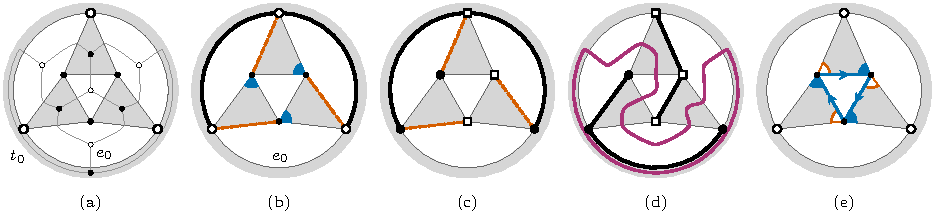
\includegraphics{figures/fig-overview.pdf}
\caption{The construction for the cube $G$ and the octahedron $T$, with $t_0$ as the outer face (grey ring). (a) $T$ with black faces shaded, the roots (circles), the side $e_0$, and $G$ in grey. (b) A good state $s$, with a wedge at each corner $s(t)$: the sides in $Q_s$ (dashed) and the two sides of $t_0$ other than $e_0$ (bold) form a spanning tree of $T$. (c) The dual spanning tree of $G$; its bold edges join the black faces (filled dots) to their children and form the matching $M$ of Lemma~\ref{lem:matching}. (d) $M^*$ (bold) and the Hamiltonian cycle $G-M$. (e) A pair $(r,s)$ (open and filled wedges) and the directed cycle formed by the edges $r(t)\to s(t)$.}
\label{fig:overview}
\end{figure}

\section{States}\label{sec:states}

We define states and prove that a good state yields a Hamiltonian cycle (Proposition~\ref{prop:recover}); this is statement~(\ref{step:cycle}) of the introduction.
All graphs are finite and simple.

\begin{definition}\label{def:euler}
An \emph{Eulerian triangulation} is a graph $T$ with at least four vertices, embedded in the sphere so that every face is bounded by a triangle, together with a colouring of its faces in black and white such that the two faces at every edge have different colours.
We write $V(t)$ for the set of the three corners of a face $t$.
The \emph{dual} $G$ of $T$ has the faces of $T$ as vertices, and every edge $f$ of $T$ has a dual edge $f^*$ joining the two faces at $f$.
For a set $N$ of edges of $T$ or of $G$, we write $N^*$ for the set of their duals.
\end{definition}

A triangulation has such a colouring if and only if its vertices have even degree.
The dual $G$ is cubic, and bipartite with the black and the white faces as its classes.
Every edge of $T$ lies on one black and one white face, so $T$ has equally many faces of each colour; if there are $n+1$ of each, then by Euler's formula
\begin{equation}\label{eq:counts}
|E(T)|=3n+3,\qquad |V(T)|=n+3,\qquad |V(G)|=2n+2 .
\end{equation}

\begin{lemma}[Plane duality]\label{lem:duality}
Let $T$ be an Eulerian triangulation with dual $G$, and let $N\subseteq E(T)$.
If $N$ contains no cycle, then $G-N^*$ is connected.
If $N$ is the edge set of a spanning tree of $T$, then $G-N^*$ is a spanning tree of $G$.
\end{lemma}

The first assertion holds because the edges of $T$ dual to a minimal nonempty edge cut of $G$ form a cycle~\cite[Proposition~4.6.1]{Diestel}, and the second follows by counting edges with~\eqref{eq:counts}.

\begin{lemma}[{\cite[Section~7]{OpenAI}}]\label{lem:dual}
Every cubic, bipartite, $3$-connected planar graph is the dual of an Eulerian triangulation.
\end{lemma}

\begin{proof}
Embed the graph $G$ in the sphere and let $T$ be its dual.
A loop or a pair of parallel edges of $T$ would be dual to an edge cut of $G$ of size at most two, and a $3$-connected graph has none; so $T$ is simple.
Its faces correspond to the vertices of $G$, so they are bounded by triangles, and the bipartition of $G$ colours them as required.
Finally $|V(T)|=|E(G)|-|V(G)|+2=\tfrac12|V(G)|+2\ge4$.
\end{proof}

\begin{setup}\label{setup}
From here until Theorem~\ref{thm:dual}, $T$ is an Eulerian triangulation with $n+1$ black faces and dual $G$, $t_0$ is a black face of $T$, and $e_0$ is a side of $t_0$.
We draw $T$ in the plane with $t_0$ as the unbounded face; so the \emph{inside} of a cycle is its bounded side, and a directed cycle runs clockwise or counterclockwise.
The three corners of $t_0$ are the \emph{roots}.
We let $A$ be the set of black faces other than $t_0$, and $X$ the set of vertices other than the roots; thus $|A|=|X|=n$ by~\eqref{eq:counts}.
\end{setup}

In this setting we look for
\begin{equation}\label{eq:aim}
\text{a perfect matching $M$ of $G$ such that $e_0^*\in M$ and $M^*$ contains no cycle.}
\end{equation}
For such an $M$ the graph $G-M$ is a spanning subgraph of $G$ with all degrees two, it is connected by Lemma~\ref{lem:duality}, and so it is a Hamiltonian cycle of $G$ that avoids $e_0^*$.

A matching as in~\eqref{eq:aim} chooses a corner in every face of $A$.
Indeed, $M^*$ is a forest with $n+1$ edges on $n+3$ vertices, so it has two components.
The Hamiltonian cycle $G-M$ crosses no edge of $M^*$, and it crosses the two sides of $t_0$ other than $e_0$, which separates the third root from the ends of $e_0$.
So deleting $e_0$ leaves three trees, one through each root.
Orient each tree towards its root.
Every vertex $x\in X$ then has one outgoing edge, which is the side in $M^*$ of exactly one face $t\in A$, and $s(t)=x$ defines a bijection $s$ from $A$ onto $X$.
The proof runs this construction backwards.

\begin{definition}\label{def:state}
A \emph{state} is a bijection $s\colon A\to X$ such that $s(t)\in V(t)$ for every $t\in A$.
Equivalently, a state is a perfect matching of the bipartite graph $H$ with classes $A$ and $X$ in which a face is adjacent to its corners in $X$.
For a state $s$, let $Q_s$ be the spanning subgraph of $T$ whose edges are the sides opposite $s(t)$ in $t$, for $t\in A$.
The state $s$ is \emph{good} if $Q_s$ together with the two sides of $t_0$ other than $e_0$ is a spanning tree $S_s$ of $T$.
\end{definition}

So $s(t)$ is to be an end of the side of $t$ in $M^*$, and $Q_s$ consists of the sides that this rules out.
An edge lies on only one black face, so $Q_s$ has $n$ edges on $n+3$ vertices, and $s$ is good if and only if $Q_s$ is a forest whose three components each contain one root.

\begin{lemma}\label{lem:outdegree}
Let $N$ be a spanning subgraph of $T$ whose edges are directed so that every vertex of $X$ has outdegree one and every root has outdegree zero.
Then every cycle of $N$ is a directed cycle.
If $N$ contains no cycle, then $N$ is a forest with three components, each containing one root.
\end{lemma}

\begin{proof}
The edges of $N$ have distinct tails, and these tails are the vertices of $X$.
So a cycle with $k$ edges has $k$ tails among its $k$ vertices and is directed, and a component of $N$ with $\nu$ vertices, $\rho$ of them roots, has $\nu-\rho$ edges; if it is a tree, then $\rho=1$.
\end{proof}

\subsection*{The disk identity}
Inside a cycle that runs through chosen corners, a state matches the black faces with vertices, which determines their number, and Euler's formula then determines the number of white faces.

\begin{lemma}[Disk identity; {\cite[Lemma~4.1]{OpenAI}}]\label{lem:disk}
Let $r$ be a state and let $C$ be a cycle of $T$ of length $h$.
For an edge $f$ of $C$ let $t_f$ be the black face at $f$, and suppose that the faces $t_f$ are distinct, that they belong to $A$, and that $r(t_f)$ is an end of $f$ for every $f$.
Let $B$ and $W$ be the numbers of black and of white faces inside $C$, and $\ell$ the number of edges $f$ of $C$ with $t_f$ inside $C$.
Then
\begin{equation}\label{eq:disk}
W=B+1\qquad\text{and}\qquad h=2\ell+3 .
\end{equation}
In particular $h$ is odd, and there is a white face inside $C$.
\end{lemma}

\begin{proof}
Let $I$ be the number of vertices inside $C$.

\step{Step 1: $B=I+\ell$.}
The vertices $r(t_f)$ are $h$ distinct vertices of $C$, so every vertex of $C$ is $r(t_f)$ for exactly one edge $f$ of $C$.
As $t_0$ is the unbounded face, the black faces inside $C$ belong to $A$ and the vertices inside $C$ to $X$.
So $r$ maps the black faces inside $C$ injectively to vertices inside or on $C$.
The image contains every vertex $x$ inside $C$, as the face $r^{-1}(x)$ at $x$ lies inside $C$, and it contains a vertex $r(t_f)$ of $C$ if and only if $t_f$ is inside $C$.

\step{Step 2: $W=B+1$.}
The part of $T$ inside and on $C$ is a plane graph with $I+h$ vertices and $B+W+1$ faces.
Each of its edges lies on one black face, which is inside $C$ except for the $h-\ell$ edges $f$ of $C$ with $t_f$ outside; so it has $3B+h-\ell$ edges.
Euler's formula $(I+h)-(3B+h-\ell)+(B+W+1)=2$ gives $W-B=1+(B-I-\ell)=1$ by Step~1.

\step{Step 3: $h=2\ell+3$.}
Counting the same edges at their white faces gives $3W+\ell$.
Hence $3B+h-\ell=3W+\ell$, that is, $h=2\ell+3(W-B)=2\ell+3$.
\end{proof}

\subsection*{From a good state to a Hamiltonian cycle}
We read off a perfect matching from the tree $S_s$ (Lemma~\ref{lem:matching}) and show that it satisfies~\eqref{eq:aim} (Proposition~\ref{prop:recover}).

\begin{lemma}\label{lem:matching}
Let $s$ be a good state.
Then $G$ has a perfect matching $M$ that contains $e_0^*$ and such that, for every $t\in A$, the side of $t$ in $M^*$ has $s(t)$ as an end.
\end{lemma}

\begin{proof}
By Lemma~\ref{lem:duality}, $Y=G-S_s^*$ is a spanning tree of $G$.
In $Y$ the vertex $t_0$ has degree one, its edge being $e_0^*$, and every $t\in A$ has degree two, since exactly one side of $t$ lies in $S_s$.
Root $Y$ at $t_0$.
Every black face then has exactly one child, every child of a black face is white, and every white face has a parent; so the edges that join the black faces to their children form a perfect matching $M$ of $G$.
It contains $e_0^*$, and for $t\in A$ the side of $t$ in $M^*$ is not in $Q_s$, so $s(t)$ is one of its ends.
\end{proof}

\begin{proposition}[{\cite[Section~6]{OpenAI}}]\label{prop:recover}
If $T$ has a good state, then $G$ has a Hamiltonian cycle that avoids $e_0^*$.
\end{proposition}

\begin{proof}
Let $s$ be a good state and $M$ the matching of Lemma~\ref{lem:matching}.
By~\eqref{eq:aim} we must show that $M^*$ is acyclic.
The reason is that the disk identity and a count of the faces that $M$ matches across a cycle of $M^*-e_0$ give different values for the surplus of white faces inside the cycle.

Direct the side of each $t\in A$ in $M^*$ away from $s(t)$.
As $s$ is a bijection onto $X$, this makes the spanning subgraph $N$ of $T$ with edge set $M^*\setminus\{e_0\}$ a directed graph as in Lemma~\ref{lem:outdegree}.
Suppose that $N$ contains a cycle $C$.
Its edges are sides of distinct faces $t\in A$, each with $s(t)$ as an end, so Lemma~\ref{lem:disk} applies with $r=s$, and~\eqref{eq:disk} gives $W-B=1$ and $h-2\ell=3$.
On the other hand, $M$ matches every face inside $C$ with a face across one of its sides.
The partner lies inside $C$ as well, unless the side is an edge of $C$; and since the edges of $C$ are in $M^*$, each of them matches the face on its inner side with the face on its outer side.
So $\ell$ black and $h-\ell$ white faces inside $C$ are matched to faces outside, and the remaining faces inside $C$ are matched in pairs of one black and one white face:
\begin{equation}\label{eq:matched}
B-\ell=W-(h-\ell),\qquad\text{that is,}\qquad W-B=h-2\ell .
\end{equation}
Hence $1=3$, a contradiction.
So $N$ contains no cycle, and by Lemma~\ref{lem:outdegree} its three components contain one root each.
As $e_0$ joins two roots, $M^*$ is acyclic.
\end{proof}

\section{Pairs of states}\label{sec:pairs}

It remains to find a good state.
Whether a state $s$ is good depends on the cycles of the undirected graph $Q_s$.
The key to the proof is a second state $r$ that differs from $s$ in every face: it directs $Q_s$ as in Lemma~\ref{lem:outdegree}, and reversing a directed cycle of $Q_s$ yields another such $r$.
For a suitable sign the two cancel, so that the states that are not good disappear from signed sums over pairs (Lemma~\ref{lem:cancel}); this is statement~(\ref{step:cancel}) of the introduction.

\begin{definition}\label{def:pair}
A \emph{pair} is an ordered pair $(r,s)$ of states with $r(t)\neq s(t)$ for every $t\in A$; for a pair, $u(t)$ denotes the third corner of $t$.
A pair directs two sides of every face $t\in A$ away from $r(t)$ (Figure~\ref{fig:example}(a)): the side in $Q_s$, from $r(t)$ to $u(t)$, and the side from $r(t)$ to $s(t)$.
The edges $r(t)\to s(t)$ form the spanning subgraph $D(r,s)$ of $T$.
As $r$ is a bijection onto $X$, both $Q_s$ and $D(r,s)$ are directed as in Lemma~\ref{lem:outdegree}.
\end{definition}


\begin{figure}[t]
\centering
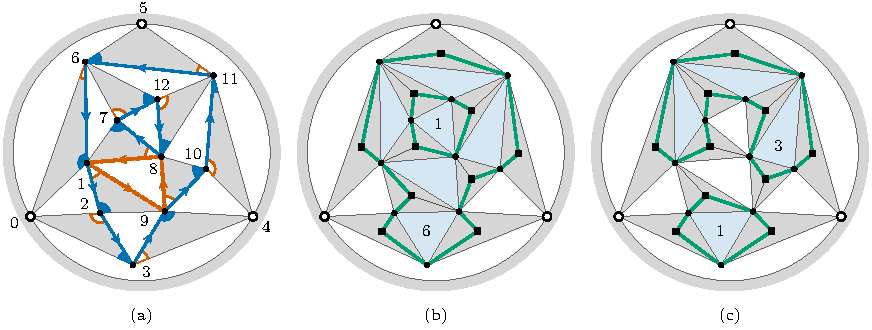
\includegraphics{figures/fig-example.pdf}
\caption{An Eulerian triangulation with $13$ vertices, roots $0,4,5$ and $n=10$. (a) A pair $(r,s)$ (open and filled wedges). The edges of $D(r,s)$ (solid arrows) form a counterclockwise cycle of length $7$ and a clockwise cycle of length $3$; the dashed arrows are the cycle of $Q_s$ through $1$, $9$ and $8$, so $s$ is not good. (b), (c) The two $2$-factors $F$ of $H$ (bold), see Section~\ref{sec:count}; the one in (b) is that of the pair in (a). The white faces inside the corresponding cycles of $D(r,s)$ are tinted, and the numbers count them; in (b) one cycle lies inside the other.}
\label{fig:example}
\end{figure}

\begin{definition}\label{def:sign}
For $t\in A$ and distinct corners $v,w$ of $t$, let $\delta_t(v,w)=1$ if $t$ lies to the left of the edge directed from $v$ to $w$, and $\delta_t(v,w)=-1$ otherwise.
The \emph{sign} of a pair $(r,s)$ is
\begin{equation}\label{eq:sign}
\eps(r,s)=\prod_{t\in A}\delta_t\bigl(r(t),s(t)\bigr).
\end{equation}
\end{definition}

Of the two corners of $t$ other than $s(t)$, one has $t$ on the left of its edge to $s(t)$ and the other on the right; so the factor of $t$ in~\eqref{eq:sign} changes when $r(t)$ is replaced by $u(t)$.

\begin{lemma}\label{lem:pair}
Let $(r,s)$ be a pair.
\begin{enumerate}
\item The state $s$ is good if and only if $Q_s$ contains no cycle.
\item Let $K$ be a cycle of $Q_s$, and let $r^K$ agree with $r$ except that $r^K(t)=u(t)$ for the faces $t$ whose side in $Q_s$ lies on $K$.
Then $(r^K,s)$ is a pair, $(r^K)^K=r$, and $\eps(r^K,s)=-\eps(r,s)$.
\end{enumerate}
\end{lemma}

\begin{proof}
(1) holds by Lemma~\ref{lem:outdegree}.
(2) By the same lemma, $K$ is a directed cycle, so both $r$ and $u$ map the faces in question bijectively onto the vertices of $K$.
Hence $r^K$ is a state, and in the pair $(r^K,s)$ the third corner of these faces is $r(t)$.
Passing from $r$ to $r^K$ changes one factor of~\eqref{eq:sign} for every edge of $K$.
The number of these edges is odd by Lemma~\ref{lem:disk}, which applies to $K$ because its edges are sides of distinct faces $t\in A$, each with $r(t)$ as an end.
\end{proof}

\begin{lemma}[Cancellation; {\cite[Lemma~5.2]{OpenAI}}]\label{lem:cancel}
For every function $f$ from the set of states to an abelian group, the sum over all pairs is the sum over the pairs whose second state is good:
\begin{equation}\label{eq:cancel}
\sum_{(r,s)}\eps(r,s)f(s)\ =\sum_{(r,s)\,:\,s\textup{ good}}\eps(r,s)f(s).
\end{equation}
\end{lemma}

\begin{proof}
For every state $s$ such that $Q_s$ contains a cycle, choose one cycle $K_s$ of $Q_s$.
By Lemma~\ref{lem:pair}(2), $r\mapsto r^{K_s}$ is an involution without fixed points on the set of states $r$ such that $(r,s)$ is a pair, and it changes $\eps(r,s)$.
So the terms with this $s$ cancel, and by Lemma~\ref{lem:pair}(1) the remaining terms are those in which $s$ is good.
\end{proof}

\section{The weighted count}\label{sec:count}

We now prove statement~(\ref{step:count}), and with it the middle implication of~\eqref{eq:chain}, by showing that the sum~\eqref{eq:cancel} is not zero for a suitable $f$.
The pairs are now grouped by the cycles of the other directed graph, $D(r,s)$.
Reversing such a cycle again changes the sign; so $f=1$ gives zero, and $f$ has to distinguish the two directions of a cycle.

\begin{definition}\label{def:factor}
In terms of the graph $H$ of Definition~\ref{def:state}, a pair $(r,s)$ consists of two disjoint perfect matchings.
Their union is a $2$-factor $F$ of $H$, the \emph{$2$-factor of the pair}, and $c(F)$ denotes the number of its cycles.
For a cycle $C$ of $T$, we let $a(C)$ be the number of white faces inside $C$.
\end{definition}

\begin{lemma}\label{lem:D}
Let $(r,s)$ be a pair with $2$-factor $F$, and let $c=c(F)$.
\begin{enumerate}
\item $D(r,s)$ consists of the three isolated roots and $c$ disjoint directed cycles whose vertex sets partition $X$.
Each of them satisfies the hypotheses of Lemma~\ref{lem:disk}; in particular $a(C)\ge1$ for every cycle $C$ of $D(r,s)$.
\item Let $C$ be a cycle of $D(r,s)$.
Exchanging $r(t)$ and $s(t)$ for the faces $t$ with a side on $C$ gives a pair with $2$-factor $F$ in which only $C$ has changed its direction; we say that it is obtained from $(r,s)$ by \emph{reversing} $C$.
The pairs with $2$-factor $F$ correspond to the $2^{c}$ choices of directions for the cycles of $D(r,s)$; without their directions these cycles depend only on $F$, and $\cC_F$ denotes their set.
\item If $c^+$ of the cycles of $D(r,s)$ run counterclockwise, then $c\equiv n\pmod 2$ and
\begin{equation}\label{eq:signformula}
\eps(r,s)=(-1)^{(n+c)/2+c^+}.
\end{equation}
\end{enumerate}
\end{lemma}

\begin{proof}
(1) In $D(r,s)$ every vertex of $X$ has outdegree one and also indegree one, because $s$ is a bijection onto $X$, and the roots are isolated.
A cycle of $F$ passes alternately through faces $t\in A$ and vertices of $X$, and the corresponding cycle of $D(r,s)$ passes through the same vertices, using the side $r(t)s(t)$ of each of these faces.
Its edges are sides of distinct faces $t\in A$, each with $r(t)$ as an end.

(2) The pairs with $2$-factor $F$ are the ways of splitting each cycle of $F$ into two perfect matchings, and reversing $C$ exchanges the two matchings of the cycle of $F$ that corresponds to $C$.

(3) Let $C$ be a cycle of $D(r,s)$, of length $h$, with $\ell$ edges whose black face is inside $C$; then $h=2\ell+3$ by~\eqref{eq:disk}.
If $C$ runs counterclockwise, its inside is on the left, and the edges of $C$ with factor $-1$ in~\eqref{eq:sign} are those whose black face is outside; there are $h-\ell=(h+3)/2$ of them.
If $C$ runs clockwise, they are the $\ell=(h-3)/2$ edges whose black face is inside.
The lengths of the cycles are odd and add up to $n$, so $c\equiv n$, and the total number of factors $-1$ is $(n-3c)/2+3c^+$, which has the parity of $(n+c)/2+c^+$.
\end{proof}

The sign formula is the disk identity $h=2\ell+3$ once more: a cycle of $D(r,s)$ has three more black faces along its outside than along its inside, so the numbers of factors $-1$ for its two directions differ by three.

We need a weight that increases by $a(C)$ when a cycle $C$ of $D(r,s)$ is turned from clockwise to counterclockwise.
It counts crossings, with signs, with arcs from the white faces to $t_0$: such an arc crosses a counterclockwise closed curve once in this count if its white face is inside the curve, and not at all otherwise.

\begin{definition}\label{def:weight}
Choose a point $p_t$ in every face $t\in A$ and join it to the corners of $t$ in $X$ by arcs inside $t$ that meet only in $p_t$ (Figure~\ref{fig:pair}(a)).
This draws $H$ in the plane, and a state $s$ is drawn as the $n$ arcs from $p_t$ to $s(t)$.

For each white face $y$ fix an arc $\gamma_y$ from a point of $y$ to a point of $t_0$ that avoids the vertices of $T$ and the points $p_t$ and crosses the arcs of $H$ transversally, in finitely many points.
For a directed curve $\alpha$ made up of arcs of $H$, let $\cross{\alpha}{\gamma_y}$ be the number of points in which $\gamma_y$ crosses $\alpha$ from the left of $\alpha$ to its right, minus the number of points in which it crosses from right to left.

For $t\in A$ and a corner $v\in X$ of $t$ put $\omega(t,v)=\sum_y\cross{p_t\to v}{\gamma_y}$, the sum being over the white faces.
The \emph{weight} of a state $s$ is
\begin{equation}\label{eq:weight}
\omega(s)=\sum_{t\in A}\omega\bigl(t,s(t)\bigr).
\end{equation}
\end{definition}

\begin{figure}[t]
\centering
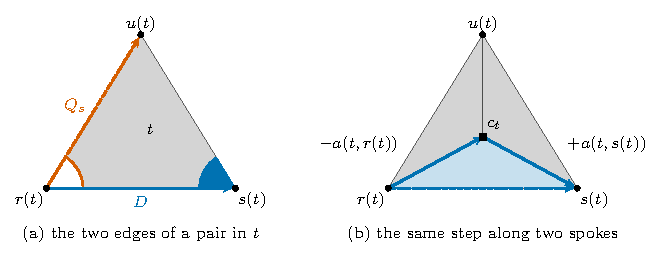
\includegraphics{figures/fig-pair.pdf}
\caption{(a) A face $t\in A$ of a pair $(r,s)$, with an open wedge at $r(t)$ and a filled wedge at $s(t)$: the edge of $D(r,s)$ (solid arrow), the side of $t$ in $Q_s$ directed by $r$ (dashed arrow), and the arcs of $H$ from the point $p_t$ to the corners of $t$ (thin lines). (b) A clockwise cycle $C$ of $D(r,s)$ in the triangulation of Figure~\ref{fig:example}, and the closed curve $\Gamma$ of Lemma~\ref{lem:weight} through the points $p_t$ (squares) of the seven black faces with a side on $C$. The six white faces inside $C$ are tinted, and the arc $\gamma_y$ from one of them to $t_0$ crosses $\Gamma$ once.}
\label{fig:pair}
\end{figure}

These weights are a variant of those of~\cite[Lemma~5.3]{OpenAI}; they are related to the height functions of perfect matchings~\cite{Thurston}.

\begin{lemma}\label{lem:weight}
Let $(r,s)$ be a pair, let $C$ be a clockwise cycle of $D(r,s)$, and let $(r',s')$ be the pair obtained by reversing $C$.
Then $\omega(s')-\omega(s)=a(C)$.
\end{lemma}

\begin{proof}
The states $s$ and $s'$ differ only on the faces $t$ with a side on $C$, where $s'(t)=r(t)$.
Let $\Gamma$ be the closed curve that runs, for each of these faces in turn, from $s(t)$ to $p_t$ and on to $r(t)$ (Figure~\ref{fig:pair}(b)).
It is obtained from $C$ by pushing every edge into its black face, and the region between an edge and its detour through $p_t$ lies in that face; so $\Gamma$ is a simple closed curve with the same white faces inside as $C$.
It runs counterclockwise, as it follows $C$ backwards.
Since reversing $\alpha$ changes the sign of $\cross{\alpha}{\gamma_y}$,
\[
\omega(s')-\omega(s)=\sum_y\ \sum_{t\,:\,r(t)s(t)\in E(C)}\Bigl(\cross{p_t\to r(t)}{\gamma_y}-\cross{p_t\to s(t)}{\gamma_y}\Bigr)=\sum_y\cross{\Gamma}{\gamma_y}.
\]
The left of $\Gamma$ is its inside, and $\gamma_y$ ends outside $\Gamma$; so $\cross{\Gamma}{\gamma_y}$ is $1$ if $y$ is inside $\Gamma$ and $0$ otherwise.
\end{proof}

With the weight as exponent, the signed sum over the pairs with a given $2$-factor factorises.

\begin{lemma}[Product formula; {\cite[(5.4)]{OpenAI}}, {\cite[(11)]{Constructive}}]\label{lem:product}
For a $2$-factor $F$ of $H$ let $\omega_F$ be the weight of the second state of the pair with $2$-factor $F$ in which all cycles of $D(r,s)$ run clockwise.
Then the Laurent polynomial $Z(z)$ defined by the sum over all pairs is also a sum over all $2$-factors of $H$:
\begin{equation}\label{eq:product}
Z(z)=\sum_{(r,s)}\eps(r,s)\,z^{\omega(s)}=\sum_{F}(-1)^{(n+c(F))/2}\,z^{\omega_F}\prod_{C\in\cC_F}\bigl(1-z^{a(C)}\bigr).
\end{equation}
\end{lemma}

\begin{proof}
Fix $F$ and let $c=c(F)$.
By Lemma~\ref{lem:D}(2), the pairs with $2$-factor $F$ arise from the one with all cycles clockwise by reversing the cycles in a subset $\mathcal J$ of $\cC_F$, one pair for each $\mathcal J$.
Such a pair has $|\mathcal J|$ counterclockwise cycles, so its sign is $(-1)^{(n+c)/2+|\mathcal J|}$ by~\eqref{eq:signformula}, and its second state has weight $\omega_F+\sum_{C\in\mathcal J}a(C)$ by Lemma~\ref{lem:weight}, applied to one cycle after another.
The sum of $(-1)^{|\mathcal J|}z^{\sum_{C\in\mathcal J}a(C)}$ over all $\mathcal J\subseteq\cC_F$ is the product in~\eqref{eq:product}.
\end{proof}

\begin{proposition}[{\cite[Proposition~5.1]{OpenAI}}, {\cite[Theorem~5.2]{Constructive}}]\label{prop:good}
If $T$ has a pair, then $T$ has a good state.
\end{proposition}

\begin{proof}
By Lemma~\ref{lem:cancel} with $f(s)=z^{\omega(s)}$, only the pairs $(r,s)$ in which $s$ is good contribute to $Z$; so it suffices to prove that $Z\neq0$.
We determine the lowest order term of $Z$ at $z=1$.
Let $m$ be the least number of cycles of a $2$-factor of $H$; there is a $2$-factor, since $T$ has a pair.
Every factor $1-z^{a}$ in~\eqref{eq:product} is $(1-z)(1+z+\dots+z^{a-1})$.
So the term of $F$ is divisible by $(1-z)^{c(F)}$, the Laurent polynomial $Z(z)$ is divisible by $(1-z)^m$, and the quotient takes at $z=1$ the value
\begin{equation}\label{eq:leading}
(-1)^{(n+m)/2}\sum_{F\,:\,c(F)=m}\ \prod_{C\in\cC_F}a(C),
\end{equation}
since the $2$-factors with more than $m$ cycles contribute zero.
By Lemma~\ref{lem:D}(1) this is a nonempty sum of positive integers, up to a sign.
Hence $Z\ne0$.
\end{proof}

Two $2$-factors whose numbers of cycles differ by two enter~\eqref{eq:product} with opposite signs, and their terms can cancel in individual coefficients.
This is why $Z$ is examined at $z=1$: there the $2$-factors with the fewest cycles dominate, and they all carry the sign $(-1)^{(n+m)/2}$.

\begin{example}\label{ex:example}
In the triangulation of Figure~\ref{fig:example}, the graph $H$ has twelve perfect matchings and two $2$-factors, each with two cycles, which enclose $6$ and $1$, respectively $3$ and $1$, white faces.
By~\eqref{eq:product}, $Z(z)=z^{\omega_0}(1-z)\bigl((1-z^6)+z^2(1-z^3)\bigr)=z^{\omega_0}\bigl(1-z+z^2-z^3-z^5+z^7\bigr)$ for some integer $\omega_0$ depending on the arcs $\gamma_y$.
The two terms $\mp z^{\omega_0+6}$, one from each $2$-factor, belong to two pairs with the same second state, which is not good, and the six remaining terms belong to six good states.
\end{example}


\section{Proof of the theorem}\label{sec:proof}

It remains to prove statement~(\ref{step:pair}), the first implication of~\eqref{eq:chain}, and to deal with separating triangles; a \emph{separating triangle} of $T$ is a triangle of $T$ that has vertices of $T$ on both of its sides.
A pair exists if and only if $H$ has a $2$-factor. This is the case if a condition of Hall type holds (Lemma~\ref{lem:flow}), and in $T$ this condition is a bound on the number of edges spanned by a set of vertices (Lemma~\ref{lem:density}).

\begin{lemma}[{\cite[(3.1)]{OpenAI}}]\label{lem:flow}
If
\begin{equation}\label{eq:hall}
\sum_{t\in A}\min\bigl(2,|V(t)\cap S|\bigr)\ \ge\ 2|S|\qquad\text{for every } S\subseteq X,
\end{equation}
then $T$ has a pair.
\end{lemma}

\begin{proof}
A $2$-factor of $H$ splits into two disjoint perfect matchings, since its cycles are even, and so gives a pair.
Consider the network with an edge of capacity $2$ from a source to every $x\in X$, an edge of capacity $1$ from $x$ to $t$ for every edge $xt$ of $H$, and an edge of capacity $2$ from every $t\in A$ to a sink.
An integral flow of value $2n$ is a $2$-factor of $H$, and it exists by the max-flow min-cut theorem~\cite{FordFulkerson}: a cut with the set $S\subseteq X$ on the side of the source has capacity at least $2(n-|S|)+\sum_{t\in A}\min(2,|V(t)\cap S|)\ge 2n$.
\end{proof}

\begin{lemma}[{\cite[(3.2)]{OpenAI}}]\label{lem:density}
For $U\subseteq V(T)$ let $e(U)$ be the number of edges with both ends in $U$, and $b(U)$ the number of black faces with all corners in $U$.
If $T$ has no separating triangle and $U$ contains the roots, then
\begin{equation}\label{eq:density}
e(U)-b(U)\le 2|U|-4 .
\end{equation}
\end{lemma}

\begin{proof}
\step{Step 1: reduction to components.}
Let $K$ be a component of the subgraph of $T$ induced by $U$, with $p$ vertices and $q$ edges, and let $b_K$ be the number of black faces of $T$ with all corners in $K$.
We show that $q-b_K\le 2p$, and that $q-b_K\le 2p-4$ if $K$ contains the roots.
This suffices, as the roots lie in one component and $b(U)$ is the sum of the numbers $b_K$.
If $p\le3$, then $q\le\binom p2\le 2p$; and if moreover $K$ contains the roots, then $K$ is the boundary of $t_0$ and $q-b_K\le 3-1$.

\step{Step 2: the triangular faces of $K$.}
Let $p\ge4$, and regard $K$ as a connected plane graph with $f$ faces.
A face of $K$ of length three is bounded by a triangle of $T$ and has the other vertices of $K$ on its far side; as this triangle is not separating, the face contains no vertex of $T$, so it is a face of $T$.
Hence the faces of $K$ of length three are the faces of $T$ with all corners in $K$, say $b_K$ black and $w_K$ white ones.

\step{Step 3: the other faces of $K$.}
Let $\Psi$ be one of the other faces of $K$, with boundary walk of length $d_\Psi\ge4$, and let $\beta_\Psi$ be the number of black faces of $T$ contained in $\Psi$ minus the number of white ones.
An edge of $T$ inside $\Psi$ lies on a black and on a white face in $\Psi$, and each of the $d_\Psi$ edges of the boundary walk lies on one face in $\Psi$; so $3\beta_\Psi$ is a sum of $d_\Psi$ terms $\pm1$.
This forces $\beta_\Psi=0$ if $d_\Psi=4$, $|\beta_\Psi|=1$ if $d_\Psi=5$, and $|\beta_\Psi|\le d_\Psi/3$ in general; in all cases $\beta_\Psi\le d_\Psi-4$.

\step{Step 4: the count.}
As $T$ has equally many black and white faces, $w_K-b_K=\sum_\Psi\beta_\Psi\le\sum_\Psi(d_\Psi-4)$.
Counting the edges of $K$ at its faces, we obtain
\[
2q=3(b_K+w_K)+\sum_\Psi d_\Psi=4f-(b_K+w_K)+\sum_\Psi(d_\Psi-4)\ \ge\ 4f-2b_K ,
\]
and $q-b_K\le 2p-4$ follows from Euler's formula $f=q-p+2$.
\end{proof}

\begin{proposition}[{\cite[Proposition~3.1]{OpenAI}}]\label{prop:pair}
If $T$ has no separating triangle, then $T$ has a pair.
\end{proposition}

\begin{proof}
We verify~\eqref{eq:hall} for $S\subseteq X$; let $U=V(T)\setminus S$.
For a black face $t$, the number of sides of $t$ with both ends in $U$, less one if all corners of $t$ are in $U$, equals $2-\min(2,|V(t)\cap S|)$.
Every edge lies on exactly one black face, and $t_0$ has no corner in $S$; summing over the $n+1$ black faces therefore gives $e(U)-b(U)=2n+2-\sum_{t\in A}\min(2,|V(t)\cap S|)$.
As $|U|=n+3-|S|$ by~\eqref{eq:counts}, the inequality~\eqref{eq:hall} is~\eqref{eq:density}.
\end{proof}

\begin{theorem}[{\cite[Corollary~7.1]{OpenAI}}, {\cite[Theorem~3]{Li}}]\label{thm:dual}
Let $T$ be an Eulerian triangulation with dual $G$, and let $e$ be an edge of $G$.
Then $G$ has a Hamiltonian cycle that does not contain $e$.
\end{theorem}

\begin{proof}
We use induction on the number of vertices of $T$.
If $T$ has no separating triangle, let $e_0$ be the edge of $T$ dual to $e$ and $t_0$ the black face at $e_0$.
Then $T$ has a pair by Proposition~\ref{prop:pair}, hence a good state by Proposition~\ref{prop:good}, and the assertion is Proposition~\ref{prop:recover}.

Now let $\Delta$ be a separating triangle of $T$, bounding the closed disks $\Delta_1$ and $\Delta_2$.
We cut $T$ along $\Delta$ into two smaller Eulerian triangulations and glue Hamiltonian cycles of their duals.
For $i=1,2$ let $T_i$ consist of the vertices and edges of $T$ in $\Delta_i$; its faces are those of $T$ in $\Delta_i$ and one new face.
As in the proof of Lemma~\ref{lem:density}, three times the difference between the numbers of black and of white faces of $T$ in $\Delta_i$ is a sum of three terms $\pm1$, one for each side of $\Delta$.
So the three faces of $T$ in $\Delta_i$ at the sides of $\Delta$ have the same colour, and giving the new face the other colour makes $T_i$ an Eulerian triangulation smaller than $T$.

The dual $G_i$ of $T_i$ is obtained from $G$ by contracting the faces of $T$ outside $\Delta_i$ to one vertex $v_i$, the new face.
The edges at $v_i$ are the duals $f_1,f_2,f_3$ of the sides of $\Delta$, which lie in both $G_1$ and $G_2$; every other edge of $G$ lies in exactly one of them.
We may assume that $e$ is an edge of $G_1$.
By induction $G_1$ has a Hamiltonian cycle $C_1$ avoiding $e$.
It contains two of the edges at $v_1$, say $f_1$ and $f_2$, and if $e$ is one of the three then $e=f_3$.
By induction, $G_2$ has a Hamiltonian cycle $C_2$ avoiding $f_3$, hence containing $f_1$ and $f_2$.
The paths $C_1-v_1$ and $C_2-v_2$, together with $f_1$ and $f_2$, form a Hamiltonian cycle of $G$ avoiding $e$.
\end{proof}

Theorem~\ref{thm:main} follows from Lemma~\ref{lem:dual} and Theorem~\ref{thm:dual}.

\section{Remarks}\label{sec:remarks}

\emph{The hypotheses.}
Bipartiteness gives the colouring of the faces of $T$, and with it the equality $|A|=|X|$ and the disk identity; Tutte's graph~\cite{Tutte} shows that it cannot be dropped.
Planarity is used throughout, and the graph found independently by Georges~\cite{Georges} and Kelmans is cubic, bipartite and $3$-connected but not Hamiltonian; see~\cite{BGM}.
$3$-connectedness enters only in Lemma~\ref{lem:dual}, to make $T$ a simple graph, and it cannot be dropped~\cite{AEHS}.

\emph{Good states.}
A good state is recovered from its matching $M$ by the construction before Definition~\ref{def:state}, so distinct good states give distinct Hamiltonian cycles.
Not every Hamiltonian cycle avoiding $e$ arises: in the hexagonal prism, four Hamiltonian cycles avoid an edge joining the two hexagons, but only two states are good.
A good state $s$ forms a pair with exactly one state, obtained by orienting the trees of $Q_s$ towards their roots~\cite[Proposition~2.1]{Constructive}; so $Z(1)=0$ counts the good states with signs, and their number is even~\cite[Theorem~5.2]{Constructive}.
The count cannot be done one $2$-factor at a time: a computer search finds an Eulerian triangulation with $16$ vertices and a $2$-factor $F$ of $H$ with a single cycle, neither of whose two pairs has a good second state.

\emph{Algorithms.}
The proof above does not construct a good state, and the manuscript~\cite{Constructive} gives two procedures that do.
The graph $H$ has at most $3^{n/2}$ perfect matchings~\cite[Lemma~6.1]{Constructive}, and a search through them finds the cycle of Theorem~\ref{thm:main} in time $3^{|V(G)|/4}$ up to a polynomial factor~\cite[Theorem~1.1]{Constructive}.
A walk on pairs that follows the two cancellations ends at a pair with good second state, after at most $2^{O(n\log n)}$ steps~\cite[Theorem~5.3]{Constructive}.
Neither bound improves on the algorithms known for Hamiltonian cycles in cubic graphs in general; see~\cite{Constructive}.
It is open whether the cycle can be found in polynomial time, and whether there are always at least $2^m$ good states, where $m$ is the least number of cycles of a $2$-factor of $H$.

\begin{thebibliography}{99}

\bibitem{ANS}
T.~Akiyama, T.~Nishizeki, and N.~Saito, \emph{NP-completeness of the Hamiltonian cycle problem for bipartite graphs}, J. Inform. Process. \textbf{3} (1980), 73--76.

\bibitem{Alt}
H.~Alt, M.~S. Payne, J.~M. Schmidt, and D.~R. Wood, \emph{Thoughts on Barnette's conjecture}, Australas. J. Combin. \textbf{64} (2016), 354--365.

\bibitem{AEHS}
T.~Asano, N.~Saito, G.~Exoo, and F.~Harary, \emph{The smallest $2$-connected cubic bipartite planar nonhamiltonian graph}, Discrete Math. \textbf{38} (1982), 1--6.

\bibitem{Barnette}
D.~W. Barnette, \emph{Conjecture 5}, Recent Progress in Combinatorics (W.~T. Tutte, ed.), Academic Press, New York, 1969, p.~343.

\bibitem{BGM}
G.~Brinkmann, J.~Goedgebeur, and B.~D. McKay, \emph{The minimality of the Georges--Kelmans graph}, Math. Comp. \textbf{91} (2022), 1483--1500.

\bibitem{Constructive}
\emph{A constructive proof of Barnette's conjecture}, anonymous unpublished manuscript, 18 October 2026.

\bibitem{Diestel}
R.~Diestel, \emph{Graph theory}, 5th ed., Graduate Texts in Mathematics, vol. 173, Springer, Berlin, 2017.

\bibitem{FederSubi}
T.~Feder and C.~Subi, \emph{On Barnette's conjecture}, Electronic Colloquium on Computational Complexity, Report TR06-015, 2006.

\bibitem{FordFulkerson}
L.~R. Ford, Jr. and D.~R. Fulkerson, \emph{Maximal flow through a network}, Canad. J. Math. \textbf{8} (1956), 399--404.

\bibitem{Georges}
J.~P. Georges, \emph{Non-Hamiltonian bicubic graphs}, J. Combin. Theory Ser. B \textbf{46} (1989), 121--124.

\bibitem{Goodey}
P.~R. Goodey, \emph{Hamiltonian circuits in polytopes with even sided faces}, Israel J. Math. \textbf{22} (1975), 52--56.

\bibitem{Hertel}
A.~Hertel, \emph{A survey and strengthening of Barnette's conjecture}, technical report, University of Toronto, 2005.

\bibitem{HineKalman}
C.~Hine and T.~K\'alm\'an, \emph{Clock theorems for triangulated surfaces}, preprint, arXiv:1808.06091, 2018.

\bibitem{HMM}
D.~A. Holton, B.~Manvel, and B.~D. McKay, \emph{Hamiltonian cycles in cubic $3$-connected bipartite planar graphs}, J. Combin. Theory Ser. B \textbf{38} (1985), 279--297.

\bibitem{Kenyon}
R.~Kenyon, \emph{Conformal invariance of loops in the double-dimer model}, Comm. Math. Phys. \textbf{326} (2014), 477--497.

\bibitem{Li}
Z.~Li, \emph{A note on the proof of Barnette's conjecture}, preprint, arXiv:2610.30490, 2026.

\bibitem{OpenAI}
OpenAI, \emph{Paired states and Hamiltonian cycles in cubic bipartite planar graphs}, preprint, 24 September 2026, \url{https://github.com/openai/math}.

\bibitem{Schnieders}
T.~Schnieders, \emph{Barnette graphs with faces up to size 8 are Hamiltonian}, preprint, arXiv:2508.03531, 2025.

\bibitem{Stein}
S.~K. Stein, \emph{B-sets and planar maps}, Pacific J. Math. \textbf{37} (1971), 217--224.

\bibitem{Thurston}
W.~P. Thurston, \emph{Conway's tiling groups}, Amer. Math. Monthly \textbf{97} (1990), 757--773.

\bibitem{Tutte}
W.~T. Tutte, \emph{On Hamiltonian circuits}, J. London Math. Soc. \textbf{21} (1946), 98--101.

\bibitem{TutteTrinity}
W.~T. Tutte, \emph{Duality and trinity}, Infinite and Finite Sets (Colloq., Keszthely, 1973), Vol.~III, Colloq. Math. Soc. J\'anos Bolyai, vol.~10, North-Holland, Amsterdam, 1975, pp.~1459--1472.

\end{thebibliography}

\end{document}
